\documentclass[a4paper, 12pt,twoside]{book}

% set the paper size and the margins
\usepackage[top = 2cm, bottom = 2cm, left = 2cm, right = 4cm ]{geometry}
\usepackage[showboxes]{textpos}
\setlength{\TPHorizModule}{10mm}
\setlength{\TPVertModule}{\TPHorizModule}
\TPMargin{2mm}
% set the header and the footnote
\usepackage{fancyhdr}
% Supress the hyphenation
\hyphenation{thatshouldnot} 
% for table and equations
\usepackage{tablefootnote}
\usepackage{amsmath,amsfonts,amsthm}
\usepackage{multirow}
\usepackage{hhline}
% make a wide hat for the least-squares regression line
 \usepackage{scalerel,stackengine}
\stackMath
\newcommand\reallywidehat[1]{%
\savestack{\tmpbox}{\stretchto{%
  \scaleto{%
    \scalerel*[\widthof{\ensuremath{#1}}]{\kern-.6pt\bigwedge\kern-.6pt}%
    {\rule[-\textheight/2]{1ex}{\textheight}}%WIDTH-LIMITED BIG WEDGE
  }{\textheight}% 
}{0.5ex}}%
\stackon[1pt]{#1}{\tmpbox}%
}
\usepackage[shortlabels]{enumitem}

% knitr packages
\usepackage[]{graphicx}
\usepackage[]{color}
%% maxwidth is the original width if it is less than linewidth
%% otherwise use linewidth (to make sure the graphics do not exceed the margin)
\makeatletter
\def\maxwidth{ %
  \ifdim\Gin@nat@width>\linewidth
    \linewidth
  \else
    \Gin@nat@width
  \fi
}
\makeatother

\definecolor{fgcolor}{rgb}{0.345, 0.345, 0.345}
\newcommand{\hlnum}[1]{\textcolor[rgb]{0.686,0.059,0.569}{#1}}%
\newcommand{\hlstr}[1]{\textcolor[rgb]{0.192,0.494,0.8}{#1}}%
\newcommand{\hlcom}[1]{\textcolor[rgb]{0.678,0.584,0.686}{\textit{#1}}}%
\newcommand{\hlopt}[1]{\textcolor[rgb]{0,0,0}{#1}}%
\newcommand{\hlstd}[1]{\textcolor[rgb]{0.345,0.345,0.345}{#1}}%
\newcommand{\hlkwa}[1]{\textcolor[rgb]{0.161,0.373,0.58}{\textbf{#1}}}%
\newcommand{\hlkwb}[1]{\textcolor[rgb]{0.69,0.353,0.396}{#1}}%
\newcommand{\hlkwc}[1]{\textcolor[rgb]{0.333,0.667,0.333}{#1}}%
\newcommand{\hlkwd}[1]{\textcolor[rgb]{0.737,0.353,0.396}{\textbf{#1}}}%
\let\hlipl\hlkwb
\usepackage{framed}
\makeatletter
\newenvironment{kframe}{%
 \def\at@end@of@kframe{}%
 \ifinner\ifhmode%
  \def\at@end@of@kframe{\end{minipage}}%
  \begin{minipage}{\columnwidth}%
 \fi\fi%
 \def\FrameCommand##1{\hskip\@totalleftmargin \hskip-\fboxsep
 \colorbox{shadecolor}{##1}\hskip-\fboxsep
     % There is no \\@totalrightmargin, so:
     \hskip-\linewidth \hskip-\@totalleftmargin \hskip\columnwidth}%
 \MakeFramed {\advance\hsize-\width
   \@totalleftmargin\z@ \linewidth\hsize
   \@setminipage}}%
 {\par\unskip\endMakeFramed%
 \at@end@of@kframe}
\makeatother


\definecolor{shadecolor}{rgb}{.97, .97, .97}
\definecolor{messagecolor}{rgb}{0, 0, 0}
\definecolor{warningcolor}{rgb}{1, 0, 1}
\definecolor{errorcolor}{rgb}{1, 0, 0}
\newenvironment{knitrout}{}{} % an empty environment to be redefined in TeX

\usepackage{alltt}


% packages will be used by the 'kable' package
\usepackage{booktabs}
\usepackage{longtable}
\usepackage{array}
\usepackage{multirow}
\usepackage[table]{xcolor}
\usepackage{wrapfig}
\usepackage{float}
\usepackage{colortbl} 
\usepackage{pdflscape}
\usepackage{tabu}
\usepackage{threeparttable}
\usepackage{threeparttablex}
\usepackage[normalem]{ulem}
\usepackage{makecell}
\usepackage{xcolor}
\IfFileExists{upquote.sty}{\usepackage{upquote}}{}

% define a color for highlight
\definecolor{asparagus}{rgb}{0.53, 0.66, 0.42}
\definecolor{babypink}{rgb}{0.96, 0.76, 0.76}
\definecolor{champagne}{rgb}{0.97, 0.91, 0.81}
\definecolor{forestgreen}{rgb}{0.13, 0.55, 0.13}
\definecolor{dollarbill}{rgb}{0.52, 0.73, 0.4}

\usepackage{tcolorbox}

\tcbset{width=0.9\textwidth,boxrule=0pt,colback=champagne,arc=0pt,
auto outer arc,left=0pt,right=0p}

\usepackage{hhline}

\usepackage{amsmath}

\setlength{\parindent}{0.5cm} 

\usepackage{siunitx}

%Chinese yen
\usepackage{stackengine}
\newcommand{\textyen}{\stackengine{-6pt}{=}{\large{\text{Y}}}{O}{c}{F}{T}{S}}

\setlength{\parindent}{0cm}

\begin{document}

%Deal with the headers of each chapter
\pagestyle{fancy}
\fancyhf{}
\renewcommand{\chaptermark}[1]{ \markboth{#1}{} }
\fancyhead[CE,CO]{\leftmark}
\fancyfoot[LE,RO]{\thepage}
\chapter{Inference about the least-squares regression line}

In chapter 2 we learned how use least-squares regression line to describe the linear relationship between two quantitative variables, based on the sampled data. Is this least-squares regression line still true for population data?  We will answer this question in this chapter.
\newpage

\section{The basics}
\begin{itemize}
   \item \textbf{Notations}\vspace{0.3cm}
   
   If the least-squares regression line is based on the sample data, the equation is 
   $$\reallywidehat{y} = a + bx$$
   If the least-squares regression line is based on the population, the corresponding parameters for statistics $a$ and $b$ are $\alpha$ and $\beta$.\vspace{0.3cm}
  
  Recall from chapter 2 that $s$ means the \textit{standard deviation of the residuals}, which is interpreted as the ``the typical error of the prediction''. The corresponding parameter is $\sigma$. \vspace{0.3cm}
  
  The least correlation $r$ is a statistic to evaluate the strength of the linear relationship. The corresponding parameter is $\rho$.\vspace{0.3cm}
  
  \item \textbf{The conditions for regression inference}\vspace{0.3cm}
  
  \begin{itemize}
    \item \textbf{Linear:} The actual relationship between $x$ and $y$ is linear. For any fixed value of $x$, the mean response my falls on the population (true) regression line $\mu_y = a + bx$.
    \item \textbf{Independent:} Individual observations are independent of each other. When sampling without replacement, check the 10\% condition.
    \item \textbf{Normal:} For any fixed value of x, the response y varies according to a  Normal distribution.
    \item \textbf{Equal SD:} The standard deviation of y (call it $\sigma$) is the same for all values of x.
     \item \textbf{Random:} The data come from a well-designed random sample or randomized experiment.
    \begin{figure}[H]
    \centering
    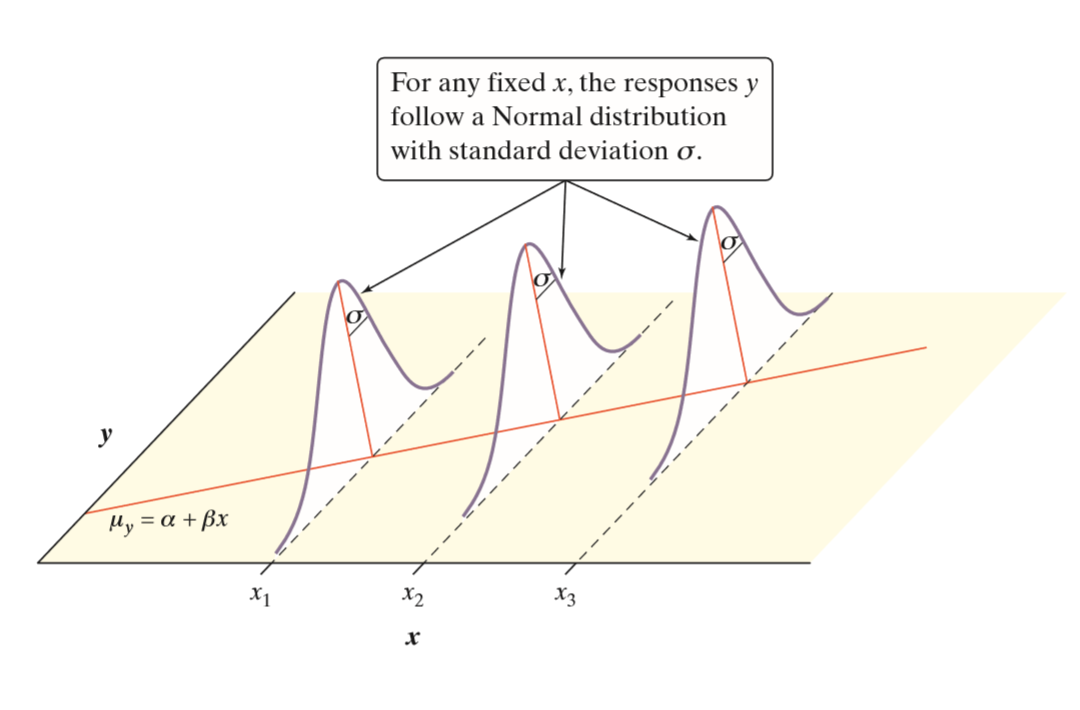
\includegraphics[scale=0.5]{InferenceForRegressionLineLinear}
    \caption[Caption for LOF]{The normal and equal SD condition   \protect\footnotemark}
    \label{InferenceForRegressionLineLinear}
    \end{figure}
    \footnotetext{This figure is adapted from \textit{The practice of statistics, 5th edition, By Starnes etc.}}
     \end{itemize} 
       
  If all the above conditions are satisfied, we can do the \textbf{regression inference}. The sampling distribution of $b$ is approximately normal.
  $$b\sim N(\mu_b, \sigma_b), \qquad \mu_b = \beta,\; \sigma_b = \frac{\sigma}{\sigma_x \sqrt{n}}$$
    
    \colorbox{babypink}{\parbox{\textwidth}{
    Those conditions are rarely checked in free response problems. In most cases, the stem of the problem tells you that all the conditions are met.
    }}
    \end{itemize}
\section{Regression inference}
   \begin{itemize}
    \item \textbf{Confidence interval about $\beta$}\vspace{0.3cm}
  \begin{textblock}{3.6}(15, -1)
  \textblockcolor{dollarbill}
  Why the the confidence interval is about $\beta$ instead of $b$?
  \end{textblock}
  
  The formula for the confidence interval  are in the same form as before.
  $$\textbf{Statistic}\pm (\textbf{Critical value})\cdot(\textbf{Standard deviation of the statistic})$$    
 
   
   From previous section we know that 
   $$\sigma_b = \frac{\sigma}{\sigma_x \sqrt{n}}.$$
   In practice, we don't know $\sigma$, and replace it by $s$. The denominator $\sigma_x\sqrt{n}$ is replaced by $s_x\sqrt{n-1}$.
   $$\textbf{SE}_b = \frac{s}{s_x\sqrt{n-1}}$$
   \vspace{0.3cm}
   
   The statistic
   $\displaystyle{t=\frac{b-\beta}{\textbf{SE}_b}}$
   has a t distribution with degree of freedom $df=n-2$.\vspace{0.3cm}
   
   Thus the formula for confidence interval is 
   $$b\pm t^* \textbf{SE}_b$$
   
   \colorbox{babypink}{\parbox{\textwidth}{
  Most of the time, $\textbf{SE}_b$ is given by the stem of the problem directly.
   }}
   
   \newpage
   \hspace{-1cm}
 \colorbox{champagne}{\parbox{\textwidth}{
 \textbf{Keep slim}\vspace{0.3cm}
 
 Does fidgeting keep you slim? Some people don’t gain weight even when they overeat. Perhaps fidgeting and other “nonexercise activity” (NEA) explain why—some people may spontaneously increase nonexercise activity when fed more. Researchers deliberately overfed a random sample of 16 healthy young adults for 8 weeks. They measured fat gain (in kilograms) as the response variable and change in energy use (in calories) from activity other than deliberate exercise\textemdash fidgeting, daily living, and the like\textemdash  as the explanatory variable. Here are the data:
 \begin{table}[H]
 \centering
 \begin{tabular}{lcccc cccc}
 \hline
 \textbf{NEA change (cal):} &−94 &−57 &−29 &135 &143 &151 &245 &355\\
 \textbf{Fat gain (kg):}& 4.2& 3.0 &3.7 &2.7 &3.2 &3.6 &2.4& 1.3\\
 \textbf{NEA change (cal):} &392& 473 &486 &535& 571 &580 &620 &690\\
 \textbf{Fat gain (kg):} &3.8 &1.7 &1.6& 2.2& 1.0 &0.4& 2.3 &1.1\\
 \hline 
 \end{tabular}
 \end{table}
 Minitab output from a least-squares regression analysis for these data is shown below.
 \begin{figure}[H]
 \centering
 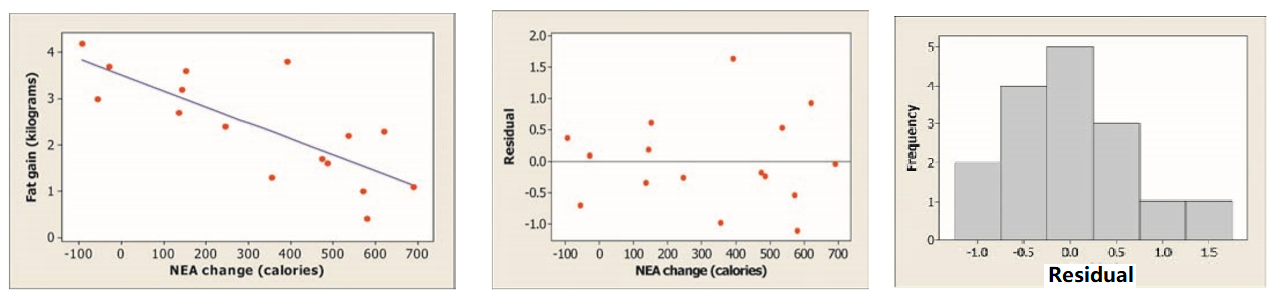
\includegraphics[scale=0.6]{Chapter9Exercise1}
 \end{figure}
  \begin{figure}[H]
 \centering
 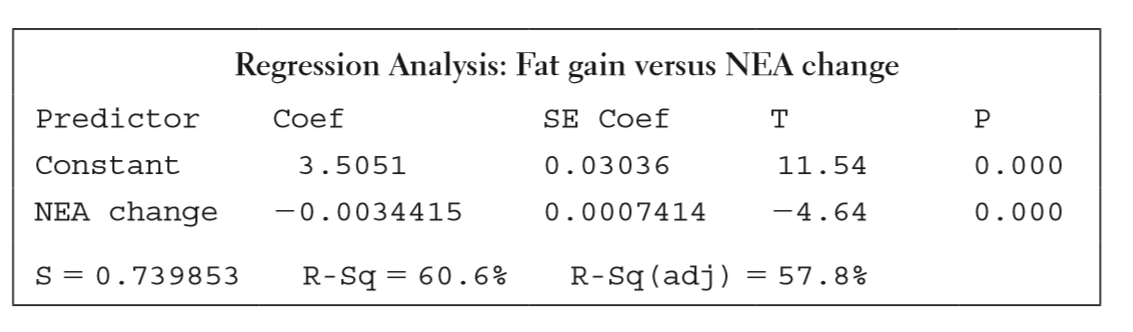
\includegraphics[scale=0.6]{Chapter9Exercise2}
 \end{figure}
 
 \begin{enumerate}[(a)]
     \item Give the standard error of the slop $\textbf{SE}_b$ and interpret this value in the context.
     \item Suppose all the conditions are met. Construct and interpret a 95\% confidence interval for the slope of the population (true) regression line.
     \item Interpret the result in (b).
     \item How would you check the \textit{normal} and \textit{equal SD} conditions?
 \end{enumerate}
 }}
 \newpage
 \item \textbf{Hypotheses test about $\beta$}  
    
    The conditions to be checked is the same as the conditions checked in constructing confidence intervals for $\beta$. \vspace{0.3cm}
    
    Suppose the null hypothesis is 
    $$\textbf{H}_0:\quad \beta = \beta_0$$
    The alternative hypothesis can be either of the following
    $$\textbf{H}_a:\quad \beta \ne \beta_0, 
    \qquad \textbf{H}_a:\quad \beta > \beta_0,
     \qquad \textbf{H}_a:\quad \beta < \beta_0$$
    The test statistic is 
     $$\displaystyle{t=\frac{b-\beta}{\textbf{SE}_b}}, \quad df = n-2$$
     The way to calculate the P-value is the same as the tests we learned before. It depend on the $\textbf{H}_a$\vspace{0.3cm}
     
     \colorbox{babypink}{\parbox{\textwidth}{
     Sometimes, you may be asked to perform a hypotheses test about population correlation $\rho$. The null hypothesis is $\textbf{H}_0:\quad \rho = 0$ and the alternative hypothesis may be either of the following
        $$\textbf{H}_a:\quad \rho \ne 0, 
    \qquad \textbf{H}_a:\quad \rho > 0,
     \qquad \textbf{H}_a:\quad \rho < 0$$
     Since we know that $\beta$ and $\rho$ have the same sign. The above hypotheses test are the same as the following:\vspace{0.3cm}
     
     The null hypothesis is $\textbf{H}_0:\quad \beta =0$. The alternative hypothesis may be either of the following:
             $$\textbf{H}_a:\quad \beta \ne 0, 
    \qquad \textbf{H}_a:\quad \beta > 0,
     \qquad \textbf{H}_a:\quad \beta < 0.$$
     }}
 \end{itemize}
\newpage
\colorbox{champagne}{\parbox{\textwidth}{
\textbf{Crying and IQ}\vspace{0.3cm}

Infants who cry easily may be more easily stimulated than others. This may be a sign of higher IQ. Child development researchers explored the relationship between the crying of infants 4 to 10 days old and their later IQ test scores. A snap of a rubber band on the sole of the foot caused the infants to cry. The researchers recorded the crying and measured its intensity by the number of peaks in the most active 20 seconds. They later measured the children’s IQ at age three years using the Stanford-Binet IQ test. A random sample of 38 infants is studied and the results are shown below.
   \begin{table}[H]
   \centering
   \begin{tabular}{|lcccc|}
   \hline
   \multicolumn{5}{|c|}{\textbf{Regression Analysis: IQ versus Crycount}}\\
   \texttt{Predictor}&\texttt{Coef}&\texttt{SE Coef}&\texttt{T}&\texttt{P}\\
   \texttt{Constant}& \texttt{ 91.268}&\texttt{ 8.934}&\texttt{ 10.22}&\texttt{ 0.000}\\
  \texttt{Crycount}&\texttt{ 1.4929}&\texttt{ 0.4870}&\texttt{ 3.07}&\texttt{ 0.004}\\
  \multicolumn{5}{|c|}{\texttt{S = 17.50  R-Sq = 20.7\%  R-Sq(adj) = 18.5\%}}\\ 
  \hline 
   \end{tabular}
   \end{table}
   
   
   \begin{enumerate}[(a)]
      \item What is the equation of the least-squares regression line for predicting IQ at age 3 from the number of crying peaks (crycount)? Interpret the slope and y intercept of the regression line in context.
      \item Interpret $s$
      \item Calculate the correlation $r$ and interpret \textit{the coefficient of determination}.
      \item Do the results provide convincing evidence of a positive linear relationship between crying counts and IQ in the population of infants? Suppose all the conditions for statistical inference are met.
   \end{enumerate}
}}
\end{document}